\section{Taking Wavelet Transforms of Inputs}\label{sec:ch6:gainlayer}

As neural network training involves presenting thousands of training samples, we
want our layer to be fast. To achieve this we would ideally choose to use a
critically sampled filter bank implementation. The fast 2-D Discrete Wavelet
Transform (DWT) is a possible option, but it has two drawbacks: it has poor
directional selectivity and any alteration of wavelet coefficients will cause
the aliasing cancelling properties of the reconstructed signal to disappear.
Instead we choose to use the $\DTCWT$ \cite{selesnick_dual-tree_2005} as at the
expense of limited redundancy (4:1), it enables us to have better directional
selectivity, and allows us to modify the wavelet coefficients and still have
minimal aliasing terms when we reconstruct \cite{kingsbury_complex_2001}.

\subsection{Aliasing in the DWT}
Consider a single level critically sampled DWT in 1-D. The aliasing cancelling
condition is:

$$G_0(z)H_0(-z) + G_1(z)H_1(-z) = 0$$

This is typically solved by using Quadrature Mirror Filters, i.e.

\begin{align}
  H_1(z) &= H_0(-z) \\
  G_0(z) &= H_0(z) \\
  G_1(z) &= -H_1(z) = -H_0(-z) 
\end{align}

\section{$\DTCWT$ Convolution}

\begin{figure}
  \centering
  \begin{tikzpicture}
    \matrix (m1) [minimum height=4mm, column sep=6mm, align=center]
	{
	%--------------------------------------------------------------------
		\node[coordinate]                  (m00) {};    &
		\node[coordinate]                  (m01) {};          &
		\node[dspsquare]                   (m02) {$A(z)$};          &
		\node[circle,draw,inner sep=1pt]   (m03) {\downsamplertext{M}}; &
		\node[dspnodeopen,dsp/label=above] (m04) {$X_a(z)$};          &
		\node[circle,draw,inner sep=1pt]   (m07) {\upsamplertext{M}}; &
		\node[dspsquare]                   (m08) {$C(z)$};          &
		\node[coordinate]                  (m09) {};          &
		\node[coordinate]                  (m0X) {};          \\
		%--------------------------------------------------------------------
		\node[dspnodefull]                 (m10) {};          &
		\node[coordinate]                  (m11) {};          &
		\node[coordinate]                  (m12) {};    &
		\node[coordinate]                  (m13) {};          &
		\node[coordinate]                  (m14) {};    &
		\node[coordinate]                  (m17) {};          &
		\node[coordinate]                  (m18) {};    &
		\node[dspadder]                    (m19) {};          &
		\node[]     (m1X) {};          \\
		%--------------------------------------------------------------------
		\node[coordinate]                  (m20) {};    &
		\node[coordinate]                  (m21) {};          &
		\node[dspsquare]                   (m22) {$B(z)$};          &
		\node[circle,draw,inner sep=1pt]   (m23) {\downsamplertext{M}}; &
		\node[dspnodeopen,dsp/label=below] (m24) {$X_b(z)$};          &
		\node[circle,draw,inner sep=1pt]   (m27) {\upsamplertext{M}}; &
		\node[dspsquare]                   (m28) {$D(z)$};          &
		\node[coordinate]                  (m29) {};          &
		\node[coordinate]                  (m2X) {};          \\
		%--------------------------------------------------------------------
	};
	\draw[dspline] (m10) -- (m11);
	\draw[dspline] (m11) -- (m01);
	\draw[dspline] (m11) -- (m21);
	\foreach \i in {0,2} {
    	\draw[dspconn] (m\i1) -- (m\i2);
    	\draw[dspconn] (m\i2) -- (m\i3);
    	\draw[dspline] (m\i3) -- (m\i4);
    	\draw[dspconn] (m\i4) -- (m\i7);
    	\draw[dspconn] (m\i7) -- (m\i8);
    	\draw[dspline] (m\i8) -- (m\i9);
	}
  \node[left=0pt of m10] (left) {$X(z)$};
  \node[below=9pt of m24] (bottom) {};
  \draw[dspconn] (m09) -- node[right, yshift=5pt] {$Y_a(z)$} (m19);
  \draw[dspconn] (m29) -- node[right, yshift=-5pt] {$Y_b(z)$} (m19);
  \draw[dspconn] (m19) -- node[right, xshift=5pt] {$Y(z)$} (m1X);
	
\end{tikzpicture}

  \mycaption{Block Diagram of 1-D $\DTCWT$}{Note the top and bottom paths are
  through the wavelet or scaling functions from just level m ($M=2^m$). Figure
  based on Figure~4 in \cite{kingsbury_complex_2001}.}
  \label{fig:ch6:dtcwt_two_tree}
\end{figure}

As we saw from \autoref{ch2:??}, if we keep only 1 passband in the $\DTCWT$ as
shown in \autoref{fig:ch6:dtcwt_two_tree} then
the end to end transfer function is:

\begin{equation}
  \frac{1}{M} \sum_{k=0}^{M-1} [A(W^kz)C(z) + B(W^kz)D(z)]
\end{equation}

Let us extend this idea to allow for any linear gain applied to the passbands
(not just zeros and ones). Ultimately, we may want to allow for nonlinear
operations applied to the wavelet coefficients, but we restrict ourselves to
linear gains so that we can build from a sensible base.

If we want to have linear gains applied to the wavelet coefficients, it would be
nice to maintain the shift invariant properties of the $\DTCWT$. 

\begin{figure}
  \centering
  \begin{tikzpicture}
    \matrix (m1) [row sep=5mm, column sep=6mm,align=center,anchor=center]
	{
	%--------------------------------------------------------------------
		\node[coordinate]                  (m00) {};    &
		\node[coordinate]                  (m01) {};          &
		\node[dspsquare]                   (m02) {$A(z)$};          &
		\node[circle,draw,inner sep=1pt]   (m03) {\downsamplertext{M}}; &
		\node[dspnodeopen,dsp/label=above] (m04) {$U_a(z)$};          &
    \node[rectangle,draw,inner sep=2pt](m05) {$G_{aa}(z)$}; &
		\node[dspnodeopen,dsp/label=above] (m06) {$V_a(z)$};          &
		\node[circle,draw,inner sep=1pt]   (m07) {\upsamplertext{M}}; &
		\node[dspsquare]                   (m08) {$C(z)$};          &
		\node[coordinate]                  (m09) {};          &
		\node[coordinate]                  (m0X) {};          \\
		%--------------------------------------------------------------------
      \node[dspnodefull]                 (m10) {};          &
		\node[coordinate]                  (m11) {};          &
		\node[coordinate]                  (m12) {};    &
		\node[coordinate]                  (m13) {};          &
		\node[coordinate]                  (m14) {};    &
		\node[coordinate]                  (m15) {};          &
		\node[coordinate]                  (m16) {};    &
		\node[coordinate]                  (m17) {};          &
		\node[coordinate]                  (m18) {};    &
		\node[dspadder]                    (m19) {};          &
    \node[]                            (m1X) {$Y(z)$};          \\
		%--------------------------------------------------------------------
		\node[coordinate]                  (m20) {};    &
		\node[coordinate]                  (m21) {};          &
		\node[dspsquare]                   (m22) {$B(z)$};          &
		\node[circle,draw,inner sep=1pt]   (m23) {\downsamplertext{M}}; &
		\node[dspnodeopen,dsp/label=below] (m24) {$U_b(z)$};          &
      \node[rectangle,draw,inner sep=2pt](m25) {$G_{bb}(z)$}; &
		\node[dspnodeopen,dsp/label=below] (m26) {$V_b(z)$};          &
		\node[circle,draw,inner sep=1pt]   (m27) {\upsamplertext{M}}; &
		\node[dspsquare]                   (m28) {$D(z)$};          &
		\node[coordinate]                  (m29) {};          &
		\node[coordinate]                  (m2X) {};          \\
		%--------------------------------------------------------------------
  };
	\draw[dspline] (m10) -- (m11);
	\draw[dspline] (m11) -- (m01);
	\draw[dspline] (m11) -- (m21);
	\foreach \i in {0,2} {
    	\draw[dspconn] (m\i1) -- (m\i2);
    	\draw[dspconn] (m\i2) -- (m\i3);
    	\draw[dspline] (m\i3) -- (m\i4);
    	\draw[dspconn] (m\i4) -- (m\i5);
    	\draw[dspline] (m\i5) -- (m\i6);
    	\draw[dspconn] (m\i6) -- (m\i7);
    	\draw[dspconn] (m\i7) -- (m\i8);
    	\draw[dspline] (m\i8) -- (m\i9);
	}
	%\draw[dspflow] (m04) --  (m06);
	%\draw[dspflow] (m24) -- (m26);
  \draw[dspconn] (m24) -- node[draw,pos=0.7,inner sep=2pt,fill=white] {$G_{ba}(z)$} (m06);
  \draw[dspconn] (m04) -- node[draw,pos=0.7,inner sep=2pt,fill=white] {$G_{ab}(z)$} (m26);
  \draw[dspconn] (m09) -- node[right] {$Y_a(z)$} (m19);
  \draw[dspconn] (m29) -- node[right] {$Y_b(z)$} (m19);
	\draw[dspconn] (m19) -- (m1X);
  \node[left=0pt of m10] (left) {$X(z)$};
  \node[below=10pt of m24] (bottom) {};
	
\end{tikzpicture}

  \mycaption{Block Diagram of 1-D $\DTCWT$}{Note the top and bottom paths are
  through the wavelet or scaling functions from just level m ($M=2^m$). Figure
  based on Figure~4 in \cite{kingsbury_complex_2001}.}
  \label{fig:ch6:dtcwt_two_tree_gain}
\end{figure}

This is a two port network with four individual transfer functions. Let us call
the transfer fucntion from $X_a$ to $Y_a$ $G_{aa}$, the transfer function from
$X_a$ to $Y_b$ $G_{ab}$, and similarly the transfer functions from $X_b$ to
$Y_a$ and $Y_b$ $G_{ba}$ and $G_{bb}$.

Then the end to end transfer function is: \textbf{FIXME}
\begin{equation}
Y(z) = Y_{a}(z) + Y_{b}(z) = \frac{1}{M} \sum_{k=0}^{M-1} X(W^k z) [A(W^kz)G(W^kz^{M})C(z) + B(W^kz)H(W^kz^{M})D(z)]
\end{equation}

If we set $H=G$ then we get:

$$Y(z) = Y_{a}(z) + Y_{b}(z) = \frac{1}{M} \sum_{k=0}^{M-1} X(W^k z)G(W^kz^{M}) [A(W^kz)C(z) + B(W^kz)D(z)]$$

And assuming the above analysis holds, we see that we are safe with aliasing, as
we know $[A(W^kz)C(z) + B(W^kz)D(z)] \approx 0$ for all $k\neq 0$. This means
that our equivalent filter becomes

\begin{eqnarray}
  Y(z) &=& \frac{1}{M} X(z)G(z^{M}) [A(z)C(z) + B(z)D(z)] \\
  &=& \frac{1}{M} X(z)G(z^{M}) [P(z)Q(z) + jP^{*}(z)Q^{*}(z)]
\end{eqnarray}

Now we know can assume that our $\DTCWT$ is well designed and extracts frequency
bands at local areas, then our filter $G(z^{M})$ allows us to modify these
passbands (e.g. by simply scaling if $G(z) = C$, or by more complex functions.


The output from \autoref{fig:dtcwt_two_tree} is:

$$ Y(z) = Y_a(z) + Y_b(z) = \frac{1}{M}\sum_{k=0}^{M-1} X\left(W^k z\right)
  \left[ A\left(W^kz\right)C(z) + B\left(W^kz\right)D(z) \right] $$

Where $W=e^{j2\pi/M}$.  To achieve shift invariance we need 
$A\left(W^kz\right)C(z) + B\left(W^kz\right)D(z)$ to be very small or to cancel
each other out for all $k \neq 0$.

The complex analysis filter (taking us into the wavelet domain) is 

$$P(z) = \frac{1}{2}\left(A(z)+jB(z)\right)$$

and the complex synthesis filter (returning us to the pixel domain) is 

$$Q(z) = \frac{1}{2}\left(C(z) - jD(z)\right)$$

where $A,B,C,D$ are real.  If $G(z) = G_r(z) + jG_i(z) = 1$ then the end-to-end
transfer function is (from section 4 of \cite{kingsbury_complex_2001}):

\begin{equation}\label{eq:end_to_end1}
\frac{Y(z)}{X(z)} = \frac{2}{M}\left(P(z)Q(z) + P^*(z)Q^*(z)\right)
\end{equation}

where $P, Q$ have support only in the top half of the Fourier plane and $P^*,
Q^*$ are $P$ and $Q$ reflected in the horizontal frequency axis. Examples of
$P(z)Q(z)$ for different subbands of a 2-D $\DTCWT$ have spectra shown in
\autoref{fig:dtcwt_bands_freq}, $P^*(z)Q^*(z)$ make up the missing half of the
frequency space.\\
\begin{tikzpicture}[%
  path image/.style={
    path picture={
      \node at (path picture bounding box.center) {
        \includegraphics[height=2.0cm]{#1}
      };
    }
  }, 
  path pic/.style={
    path picture={
      \node at (path picture bounding box.center) {
        \includegraphics[height=1.2cm]{#1}
      };
    }
  }, 
  path pic2/.style={
    path picture={
      \node at (path picture bounding box.center) {
        \includegraphics[height=0.8cm]{#1}
      };
    }
  }, 
  scale=0.6]

  \tikzcuboid{
  shiftx=-1.5cm,
  shifty=-2.5cm,
  scale=0.5,
  anglex=0, 
  angley=90, 
  anglez=230,
  dimx=3, 
  dimy=3, 
  dimz=6,
  densityx=1, 
  densityy=1, 
  densityz=1,
  shade=false,
  emphedge=true,
  shadeopacity=0,
  emphstyle/.style={rounded corners=0.2pt,line width=0.3mm},
  front/.style={draw=blue!50!white,fill=blue!50!white},%
  right/.style={draw=blue!50!white,fill=blue!50!white},%
  top/.style={draw=blue!50!white,fill=blue!50!white},%
  drawxdims=true,
  dimxval=W,
  drawydims=true,
  dimyval=H,
  drawzdims=true,
  dimzval=C_l,
  }
  \draw (0, .3, 0) node {\large{$x^{(l)}$}};
  \draw [path image=\imgpath/waveys.png, draw=black] (1.5,1.5,0) rectangle (6,0,0);
  \draw (3.75, 1.9, 0) node {\large{$\psi_{j, \theta}$}};
  \draw (1.5,0,0) -- (3,-1.7,0);
  \draw (6,0,0) -- (3.3,-1.7,0);
  \draw [path pic2=\imgpath/lowpass.png, draw=black] (2.5,-2.5,10) rectangle (3.5,-1.5,10);
  \draw (3, -1.1, 10) node {\large{$\phi_{j}$}};
  \draw (3.5,-1.5,10) -- (3.5,-1.7,8);

  % \draw (2.4, -1.5, 0) node {\Large{$\conv$}};
  \draw (2.5, -1.5, 3) node {\Large{$\conv$}};
  \draw [->, fill=gray!30,ultra thick] (4, -1.5, 0) -- (5, -1.5, 0);
  \draw [->, fill=gray!30,ultra thick] (4.5, -1.5, 9) -- (5.85, -1.5, 11);

  \tikzcuboid{
  shiftx=3cm,
  shifty=-1.7cm,
  shiftz=0,
  scale=0.3,
  dimx=1, dimy=1, dimz=4,
  densityx=2, densityy=2, densityz=2,
  drawxdims=false,
  drawydims=false,
  drawzdims=true,
  dimzval=12,
  front/.style={draw=yellow!70!white,fill=yellow!70!white},%
  right/.style={draw=yellow!70!white,fill=yellow!70!white},%
  top/.style={draw=yellow!70!white,fill=yellow!70!white},%
  }
  \tikzcuboid{
  shiftz=8/0.3,
  scale=0.3,
  dimx=1, dimy=1, dimz=1,
  densityx=2, densityy=2, densityz=2,
  drawxdims=false,
  drawydims=false,
  drawzdims=false,
  }


  \tikzcuboid{
  shiftx=6cm,
  shifty=-2.0cm,
  shiftz=0.8cm,
  scale=0.5,
  dimx=2, dimy=2, dimz=4,
  densityx=4, densityy=4, densityz=2,
  drawzdims=true,
  dimzval=C_l,
  front/.style={draw=blue!50!white,fill=blue!50!white},%
  right/.style={draw=blue!50!white,fill=blue!50!white},%
  top/.style={draw=blue!50!white,fill=blue!50!white},%
  }

  \tikzcuboid{
  shiftx=6cm,
  shifty=-2cm,
  shiftz=0cm,
  scale=0.5,
  dimx=2, dimy=2, dimz=24,
  densityx=2, densityy=2, densityz=2,
  drawxdims=true,
  dimxval=\frac{W}{2},
  drawydims=true,
  dimyval=\frac{H}{2},
  drawzdims=true,
  dimzval=12C_l,
  front/.style={draw=blue!50!white,fill=blue!50!white},%
  right/.style={draw=blue!50!white,fill=blue!50!white},%
  top/.style={draw=blue!50!white,fill=blue!50!white},%
  }

  % \draw [->, fill=gray!30,ultra thick] (8.5, -1.5, 0) -- (10.5, -1.5, 0) node[midway, above] (mag) {\large{$\lvert\cdot\rvert$}};
  \draw [->, fill=gray!30,ultra thick] (8.5, -1.5, 0) -- (10.5, -1.5, 0) node[midway, above] (mag) {\Large{ $\lvert \cdot \rvert$} };
  \draw [path pic=\imgpath/mag.png, draw=white] (9.25,0,0) rectangle (11.75,2,0);
  \draw (9.25,0,0) -- (mag.north);
  \draw (11.75,0,0) -- (mag.north);
  \draw[->, fill=gray!30, ultra thick] (8.5, -2, 10) -- (10, -3, 3);

  \tikzcuboid{
  shiftx=11.5cm,
  shifty=-2cm,
  scale=0.5,
  dimx=2, dimy=2, dimz=12,
  densityx=2, densityy=2, densityz=2,
  dimzval=6C_l,
  drawxdims=false,
  drawydims=false,
  front/.style={draw=blue!50!white,fill=blue!50!white},%
  right/.style={draw=blue!50!white,fill=blue!50!white},%
  top/.style={draw=blue!50!white,fill=blue!50!white},%
  }
  \tikzcuboid{
  shiftx=11.5cm,
  shifty=-2cm,
  shiftz=8,
  scale=0.5,
  drawxdims=true,
  drawydims=true,
  dimx=2, dimy=2, dimz=4,
  densityx=2, densityy=2, densityz=2,
  dimzval=C_l,
  front/.style={draw=blue!50!white,fill=blue!50!white},%
  right/.style={draw=blue!50!white,fill=blue!50!white},%
  top/.style={draw=blue!50!white,fill=blue!50!white},%
  }
  \draw (13.2, 0.8, 0) node {\large{$z^{(l+1)}$}};
  \draw (20.5, 0.3, 0) node {\large{$y^{(l+1)}$}};
  \draw (24.5, 0.3, 0) node {\large{$x^{(l+1)}$}};
  \draw (14, -1.5, 0) node {\Large{$\conv$}};

  \tikzcuboid{
  shiftx=15.2cm,
  shifty=-1.0cm,
  shiftz=0,
  scale=0.5,
  dimx=0.4, dimy=0.4, dimz=14,
  densityx=5, densityy=5, densityz=2,
  drawxdims=false,
  drawydims=false,
  drawzdims=false,
  front/.style={draw=red!50!white,fill=red!50!white},%
  right/.style={draw=red!50!white,fill=red!50!white},%
  top/.style={draw=red!50!white,fill=red!50!white},%
  }
  \tikzcuboid{
  shifty=-1.65cm,
  }
  \tikzcuboid{
  shifty=-3.0cm,
  scale=0.5,
  drawxdims=true,
  dimxval=1,
  drawydims=true,
  dimyval=1,
  drawzdims=true,
  dimzval=7C_l,
  }
  \draw (15.5, -1.8, 0) node {$\vdots$};
  \draw [<->] (15.7, -0.8, -3) -- (15.7, -3, -3) node[near start, right] {$C_{l+1}$};
  \draw [->, fill=gray!30,ultra thick] (17.5, -1.5, 0) -- (18.5, -1.5, 0);

  \tikzcuboid{
  shiftx=19.5cm,
  shifty=-2.25cm,
  scale=0.5,
  dimx=2, dimy=2, dimz=6,
  densityx=4, densityy=4, densityz=2,
  drawzdims=false,
  drawxdims=false,
  drawydims=false,
  front/.style={draw=blue!50!white,fill=blue!50!white},%
  right/.style={draw=blue!50!white,fill=blue!50!white},%
  top/.style={draw=blue!50!white,fill=blue!50!white},%
  }
  \draw [->, fill=gray!30,ultra thick] (21.5, -1.5, 0) -- (22.5, -1.5, 0)
    node[midway, above] {$\sigma$};

  \tikzcuboid{
  shiftx=23.5cm,
  shifty=-2.25cm,
  scale=0.5,
  dimx=2, dimy=2, dimz=6,
  densityx=4, densityy=4, densityz=2,
  drawzdims=true,
  dimzval=C_{l+1},
  drawxdims=true,
  dimxval=\frac{W}{2},
  drawydims=true,
  dimyval=\frac{H}{2},
  front/.style={draw=blue!50!white,fill=blue!50!white},%
  right/.style={draw=blue!50!white,fill=blue!50!white},%
  top/.style={draw=blue!50!white,fill=blue!50!white},%
  }

\end{tikzpicture}




\subsection{Forward propagation}
\autoref{fig:ch6:fwd_bwd} shows the block diagram using $Z$-transforms for
a single band of our system (it is based on Figure~4 in
\cite{kingsbury_complex_2001}). To keep things simple for the rest of
\autoref{sec:ch6:method} the figure shown is for a 1-D system; it is relatively
straightforward to extend this to 2-D\cite{selesnick_dual-tree_2005}. The
complex analysis filter (taking us into the wavelet domain) is $P(z)
= \frac{1}{2}\left(A(z)+jB(z)\right)$ and the complex synthesis filter
(returning us to the pixel domain) is $Q(z) = \frac{1}{2}\left(C(z)
  - jD(z)\right)$ where $A,B,C,D$ are real.  If $G(z) = G_r(z) + jG_i(z) = 1$
  then the end-to-end transfer function is (from section 4 of
\cite{kingsbury_complex_2001}):

\begin{equation}\label{eq:ch6:end_to_end1}
\frac{Y(z)}{X(z)} = \frac{2}{M}\left(P(z)Q(z) + P^*(z)Q^*(z)\right)
\end{equation}

where $P, Q$ have support only in the top half of the Fourier plane and $P^*,
Q^*$ are $P$ and $Q$ reflected in the horizontal frequency axis. Examples of
$P(z)Q(z)$ for different subbands of a 2-D $\DTCWT$ have spectra shown in
\autoref{fig:ch6:dtcwt_bands_freq}, $P^*(z)Q^*(z)$ make up the missing half of
the frequency space.\\ 

Modifying this from the standard wavelet equations by
adding the subband gains $G_r(z)$ and $G_i(z)$, the transfer function becomes:
\begin{equation}\label{eq:ch6:end_to_end2}
    \frac{Y(z)}{X(z)} = \frac{2}{M} \left[ \right. G_r(z^M) \left( P(z)Q(z) + P^*(z)Q^*(z) \right) +  
      \left. jG_i(z^M) \left(P(z)Q(z)-P^*(z)Q^*(z) \right) \right]
\end{equation}

\subsection{Backpropagation}
We start with the commonly known property that for a convolutional block, the
gradient with respect to the input is the gradient with respect to the output
convolved with the time reverse of the filter. More formally, if 
$Y(z) = H(z) X(z)$:
\begin{equation}\label{eq:ch6:backprop}
\Delta X(z) = H(z^{-1}) \Delta Y(z)
\end{equation}
where $H(z^{-1})$ is the $Z$-transform of the time/space reverse of $H(z)$,
$\Delta Y(z) \triangleq \dydx{L}{Y}(z)$ is the gradient of the loss with respect
to the output, and $\Delta X(z) \triangleq \dydx{L}{X}(z)$ is the gradient of
the loss with respect to the input. If H were complex, the first term in
\autoref{eq:ch6:backprop} would be $\bar{H}(1/\bar{z})$, but as each individual
block in the $\DTCWT$ is purely real, we can use the simpler form. 

Assume we already have access to the quantity $\Delta Y(z)$ (this is the input
to the backwards pass). \autoref{fig:ch6:bwd_pass} illustrates the
backpropagation procedure. An interesting result is that the backwards pass of
an inverse wavelet transform is equivalent to doing a forward wavelet
transform.\footnote{As shown in \autoref{fig:ch6:bwd_pass}, the analysis and
synthesis filters have to be swapped and time reversed. For orthogonal wavelet
transforms, the synthesis filters are already the time reverse of the analysis
filters, so no change has to be done. The q-shift filters of the $\DTCWT$
\cite{kingsbury_design_2003} have this property.} Similarly, the backwards pass
of the forward transform is equivalent to doing the inverse transform. The
weight update gradients are then calculated by finding 
$\Delta W(z) = \DTCWT\left\{ \Delta Y(z) \right\}$ and then convolving with the 
time reverse of the saved wavelet coefficients from the forward pass - $V(z)$.

\begin{gather}
  \Delta G_r(z) = \Delta W_r(z) V_r(z^{-1}) + \Delta W_i(z) V_i(z^{-1})  \label{eq:ch6:gr_update}\\
  \Delta G_i(z) =  -\Delta W_r(z) V_i(z^{-1}) + \Delta W_i(z) V_r(z^{-1})  \label{eq:ch6:gi_update} 
\end{gather}

Unsurprisingly, the passthrough gradients have similar form to
\autoref{eq:ch6:end_to_end2}:
\begin{equation}\label{eq:ch6:passthrough}
    \Delta X(z) = \frac{2\Delta Y(z)}{M} \left[G_r(z^{-M})\left( PQ + P^*Q^* \right)\right. + 
      \left. jG_i(z^{-M}) \left(PQ-P^*Q^* \right) \right] 
\end{equation}
where we have dropped the $z$ terms on $P(z), Q(z), P^*(z), Q^*(z)$ for brevity.

Note that we only need to evaluate equations
~\ref{eq:ch6:gr_update},\ref{eq:ch6:gi_update},\ref{eq:ch6:passthrough} over the
support of $G(z)$ i.e., if it is a single number we only need to calculate
$\left.\Delta G(z)\right\rvert_{z=0}$.


\subsection{Memory Cost}
Again considering a two scale transform --- instead of learning $w\in \reals[F
\x C\x K\x K]$ we learn complex gains at the two scales, and a real gain for the
real lowpass:

\begin{eqnarray*}
  g_1 &\in& \complexes[F\x C\x 6\x 1\x 1] \\
  g_2 &\in& \complexes[F\x C\x 6\x 1\x 1] \\
  g_{lp} &\in& \reals[F\x C\x 1\x 1]
\end{eqnarray*}

We have set the spatial dimension to be $1\x 1$ to show that this gain is
identical to a $1\x 1$ convolution over the complex wavelet coefficients. If we
wish, we can learn larger spatial sizes to have more complex
attenuation/magnification of the subbands. We also can use more/fewer than
2 wavelet scales.  At first glance, we have increased our parameterization by
a factor of 25 (13 subbands, of which all but the lowpass are complex), but
each one of these gains affects a large spatial size. For the first scale, the
effective size is about $5\x 5$ pixels, for the second scale it is about $15\x
15$.

\subsection{Computational Cost}
A standard convolutional layer needs $K^2 F$ multiplies per input pixel (of
which there are $C\x H\x W$). In comparison, the wavelet gain method does a set
number of operations per pixel for the forward and inverse transforms, and then
applies gains on subsampled activations. For a 2 level $\DTCWT$ the transform
overhead is about 60 multiplies for both the forward and inverse transform. It
is important to note that unlike the filtering operation, this does not scale
with $F$. The learned gains in each subband do scale with the number of output
channels, but can have smaller spatial size (as they have larger effective
sizes) as well as having fewer pixels to operate on (because of the decimation).
The end result is that as $F$ and $C$ grow, the overhead of the $C$ forward and
$F$ inverse transforms is outweighed by cost of $FC$ mixing processes, which
should in turn be significantly less than the cost of $FC$ $K\x K$ standard
convolutions for equivalent spatial sizes.

\begin{figure}[ht]
  \centering
  % \subfloat[]{%
    % 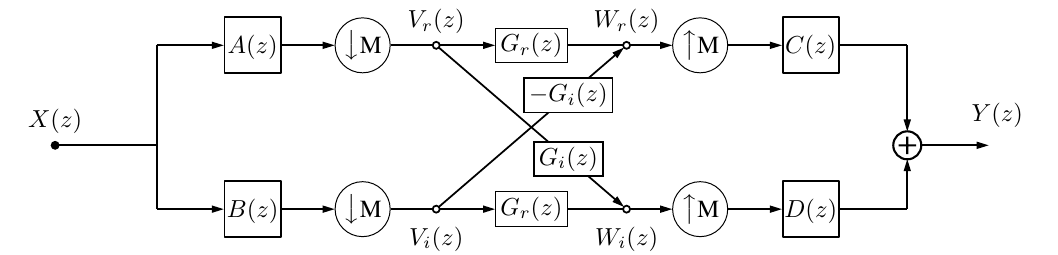
\includegraphics[width=.85\textwidth]{freqlearn/images/top_block.png}
    % \label{fig:ch6:fwd_pass}
  % }
   % \newline
  % \subfloat[]{%
    % 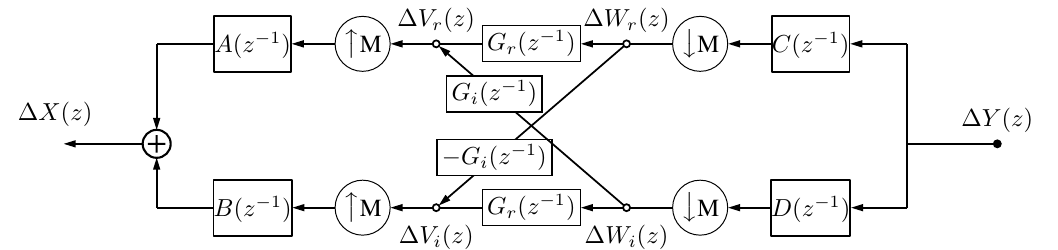
\includegraphics[width=.85\textwidth]{freqlearn/images/bottom_block.png}
    % \label{fig:ch6:bwd_pass}
  % }
  \makebox[\textwidth][c]{%
    \resizebox{1.1\textwidth}{!}{\begin{tikzpicture}
    \matrix (m1) [row sep=5mm, column sep=6mm,align=center,anchor=center]
	{
	% %--------------------------------------------------------------------
		% \node[coordinate]                  (m00) {};    &
		% \node[coordinate]                  (m01) {};          &
		% \node[dspsquare]                   (m02) {$A(z)$};          &
		% \node[circle,draw,inner sep=1pt]   (m03) {\downsamplertext{M}}; &
		% \node[dspnodeopen,dsp/label=above] (m04) {$V_r(z)$};          &
		% \node[rectangle,draw,inner sep=2pt](m05) {$G_r(z)$}; &
		% \node[dspnodeopen,dsp/label=above] (m06) {$W_r(z)$};          &
		% \node[circle,draw,inner sep=1pt]   (m07) {\upsamplertext{M}}; &
		% \node[dspsquare]                   (m08) {$C(z)$};          &
		% \node[coordinate]                  (m09) {};          &
		% \node[coordinate]                  (m0X) {};          \\
		% %--------------------------------------------------------------------
		% \node[]                            (m10) {$X(z)$};          &
		% \node[coordinate]                  (m11) {};          &
		% \node[coordinate]                  (m12) {};    &
		% \node[coordinate]                  (m13) {};          &
		% \node[coordinate]                  (m14) {};    &
		% \node[coordinate]                  (m15) {};          &
		% \node[coordinate]                  (m16) {};    &
		% \node[coordinate]                  (m17) {};          &
		% \node[coordinate]                  (m18) {};    &
		% \node[dspadder]                    (m19) {};          &
    % \node[]                            (m1X) {$Y(z)$};          \\
		% %--------------------------------------------------------------------
		% \node[coordinate]                  (m20) {};    &
		% \node[coordinate]                  (m21) {};          &
		% \node[dspsquare]                   (m22) {$B(z)$};          &
		% \node[circle,draw,inner sep=1pt]   (m23) {\downsamplertext{M}}; &
		% \node[dspnodeopen,dsp/label=below] (m24) {$V_i(z)$};          &
		% \node[rectangle,draw,inner sep=2pt](m25) {$G_r(z)$}; &
		% \node[dspnodeopen,dsp/label=below] (m26) {$W_i(z)$};          &
		% \node[circle,draw,inner sep=1pt]   (m27) {\upsamplertext{M}}; &
		% \node[dspsquare]                   (m28) {$D(z)$};          &
		% \node[coordinate]                  (m29) {};          &
		% \node[coordinate]                  (m2X) {};          \\
		% %--------------------------------------------------------------------
		% &&&&&&&&& \\
		\node[coordinate]                  (m00a) {};    &
		\node[coordinate]                  (m01a) {};          &
		\node[dspsquare]                   (m02a) {$A\left(z^{-1}\right)$};          &
		\node[circle,draw,inner sep=1pt]   (m03a) {\upsamplertext{M}}; &
		\node[dspnodeopen,dsp/label=above] (m04a) {$\Delta U_r(z)$};          &
		%\node[coordinate]                  (m05) {}; &
		\node[rectangle,draw,inner sep=2pt](m05a) {$G_r\left(z^{-1}\right)$}; &
		\node[dspnodeopen,dsp/label=above] (m06a) {$\Delta V_r(z)$};          &
		\node[circle,draw,inner sep=1pt]   (m07a) {\downsamplertext{M}}; &
		\node[dspsquare]                   (m08a) {$C\left(z^{-1}\right)$};          &
		\node[coordinate]                  (m09a) {};          &
		\node[coordinate]                  (m0Xa) {};          \\
		%--------------------------------------------------------------------
		%\node[coordinate]  (m10) {$\Delta X(z)$};          &
    \node[]                            (m10a) {$\Delta X(z)$}; &
		\node[dspadder]                    (m11a) {};          &
		\node[coordinate]                  (m12a) {};    &
		\node[coordinate]                  (m13a) {};          &
		\node[coordinate]                  (m14a) {};    &
		\node[coordinate]                  (m15a) {};          &
		\node[coordinate]                  (m16a) {};    &
		\node[coordinate]                  (m17a) {};          &
		\node[coordinate]                  (m18a) {};    &
		\node[coordinate]                  (m19a) {};          &
		\node[]                            (m1Xa) {$\Delta Y(z)$};          \\
		%--------------------------------------------------------------------
		\node[coordinate]                  (m20a) {};    &
		\node[coordinate]                  (m21a) {};          &
		\node[dspsquare]                   (m22a) {$B\left(z^{-1}\right)$};          &
		\node[circle,draw,inner sep=1pt]   (m23a) {\upsamplertext{M}}; &
		\node[dspnodeopen,dsp/label=below] (m24a) {$\Delta U_i(z)$};          &
		%\node[coordinate]                  (m25) {}; &
		\node[rectangle,draw,inner sep=2pt](m25a) {$G_r\left(z^{-1}\right)$}; &
		\node[dspnodeopen,dsp/label=below] (m26a) {$\Delta V_i(z)$};          &
		\node[circle,draw,inner sep=1pt]   (m27a) {\downsamplertext{M}}; &
		\node[dspsquare]                   (m28a) {$D\left(z^{-1}\right)$};          &
		\node[coordinate]                  (m29a) {};          &
		\node[coordinate]                  (m2Xa) {};          \\
		%--------------------------------------------------------------------
	};
	% \draw[dspline] (m10) -- (m11);
	% \draw[dspline] (m11) -- (m01);
	% \draw[dspline] (m11) -- (m21);
	% \foreach \i in {0,2} {
      % \draw[dspconn] (m\i1) -- (m\i2);
      % \draw[dspconn] (m\i2) -- (m\i3);
      % \draw[dspline] (m\i3) -- (m\i4);
      % \draw[dspconn] (m\i4) -- (m\i5);
      % \draw[dspline] (m\i5) -- (m\i6);
      % \draw[dspconn] (m\i6) -- (m\i7);
      % \draw[dspconn] (m\i7) -- (m\i8);
      % \draw[dspline] (m\i8) -- (m\i9);
	% }
	% %\draw[dspflow] (m04) --  (m06);
	% %\draw[dspflow] (m24) -- (m26);
	% \draw[dspconn] (m24) -- node[draw,pos=0.7,inner sep=2pt,fill=white] {$-G_i(z)$} (m06);
	% \draw[dspconn] (m04) -- node[draw,pos=0.7,inner sep=2pt,fill=white] {$G_i(z)$} (m26);
	% \draw[dspconn] (m09) -- (m19);
	% \draw[dspconn] (m29) -- (m19);
	% \draw[dspconn] (m19) -- (m1X);
	\draw[dspconn] (m11a) -- (m10a);
	\draw[dspconn] (m01a) -- (m11a);
	\draw[dspconn] (m21a) -- (m11a);
	\foreach \i in {0,2} {
    	\draw[dspconn] (m\i9a) -- (m\i8a);
    	\draw[dspconn] (m\i8a) -- (m\i7a);
    	\draw[dspline] (m\i7a) -- (m\i6a);
    	\draw[dspconn] (m\i6a) -- (m\i5a);
    	\draw[dspline] (m\i5a) -- (m\i4a);
    	\draw[dspconn] (m\i4a) -- (m\i3a);
    	\draw[dspconn] (m\i3a) -- (m\i2a);
    	\draw[dspline] (m\i2a) -- (m\i1a);
	}
	%\draw[dspflow] (m04) --  (m06);
	%\draw[dspflow] (m24) -- (m26);
	\draw[dspconn] (m06a) -- node[draw,pos=0.7,inner sep=2pt,fill=white] {$-G_i\left(z^{-1}\right)$} (m24a);
	\draw[dspconn] (m26a) -- node[draw,pos=0.7,inner sep=2pt,fill=white] {$G_i\left(z^{-1}\right)$} (m04a);
	\draw[dspline] (m09a) -- (m19a);
	\draw[dspline] (m29a) -- (m19a);
	\draw[dspline] (m19a) -- (m1Xa);
	
\end{tikzpicture}
}
  }
  \mycaption{Forward and backward block diagrams for $\DTCWT$ gain layer}{Based
    on Figure~4 in \cite{kingsbury_complex_2001}. Ignoring the $G$ gains, the
    top and bottom paths (through $A, C$ and $B, D$ respectively) make up the
    the real and imaginary parts for \emph{one subband} of the dual tree system.
    Combined, $A+jB$ and $C-jD$ make the complex filters necessary to have
    support on one side of the Fourier domain (see
    \autoref{fig:ch6:dtcwt_bands}). Adding in the complex gain $G_r + jG_i$, we
    can now attenuate/shape the impulse response in each of the subbands. To
    allow for learning, we need backpropagation. The bottom diagram indicates
    how to pass gradients $\Delta Y(z)$ through the layer. Note that upsampling
    has become downsampling, and convolution has become convolution with the
  time reverse of the filter (represented by $z^{-1}$ terms).}
  \label{fig:ch6:fwd_bwd}
\end{figure}




\subsection{Examples}
\autoref{fig:ch6:example_impulses} show example impulse responses of our layer.
These impulses were generated by randomly initializing both the real and
imaginary parts of $g_2 \in \complexes[6\x 1\x 1]$ from $\mathcal{N}(0,1)$ and
$g_1, g_{lp}$ are set to 0. I.e. each shape has 12 random variables. It is good
to see that there is still a large degree of variability between shapes. Our
experiments have shown that the distribution of the normalized cross-correlation
between 512 of such randomly generated shapes matches the distribution for
random vectors with roughly 11.5 degrees of freedom.

